\documentclass[a4paper,11pt,twocolumn]{article}

\usepackage{icphs2015}
\usepackage{metalogo} % Only needed for the XeLaTeX logo

\title{Attention, word position, and perceptual learning}
\author{XXX and XXX}
\organization{XXX}
\email{XXX and XXX}
\begin{document}

\maketitle

\begin{abstract}
This paper presents the results of an experiment which tested the roles of directed attention and lexical bias on perceptual learning. Attention was manipulated by directing a group of listeners to be aware the speaker had an ambiguous pronunciation of /s/. Lexical bias was manifested by where in the word the ambiguous /s/ was positioned -- the first or final syllable. In all conditions listeners were exposed to an ambiguous sound halfway between an /s/ and a /ʃ/ in word contexts for /s/.  Listeners who were only exposed to the ambiguous sound in final syllable adapted their category boundary more than listeners who were exposed to the ambiguous sound at the beginnings of words, but only when they were not explicitly instructed to pay attention to the speaker's ambiguous /s/ sounds. These results indicate that perceptual adaptation is at least a partially controlled adjustment. 
\end{abstract}

\keywords{perceptual learning, lexical bias, attention}


\section{Introduction}

Perceptual learning in speech perception is a robust phenomenon whereby listeners exposed to a novel characteristic of a speaker adapt their perceptual system to that characteristic. For instance, if a speaker produces /s/ or /f/ in a way that sounds more like the other, and the context is clear what the intended production was (i.e., in a word environment \cite{Norris2003} or synchronous with a video contextualizing place of articulation \cite{Bertelson2003}), listeners will expand the intended category at the expense of the other.  The context that these ambiguous sounds are embedded in is crucial; perceptual learning does not occur with nonwords \cite{Norris2003}. Adaptation to unfamiliar accents in sentence contexts has also been documented \cite{Bradlow2008}.

Research on perceptual learning has focused on the ability or inability of listeners to generalize from exposure to categorization.  Perceptual learning seems to generalize more as the similarity between the exposure and test stimuli increases. Perceptual learning of voicing contrasts generalize across speakers \cite{Kraljic2007}, and sibilant categories generalize across speakers when the exposure distributions and test distributions overlap naturally \cite{Kraljic2005} or artificially \cite{Eisner2006}. Exposure in one language can also cause perceptual learning in another \cite{Reinisch2013}.  There is conflicting evidence as to whether exposure to speaker-specific cues to major class features can cause perceptual learning for categories beyond the original exposure categories \cite{Kraljic2006,Reinisch2014}.  

In all of these studies, the ambiguous sounds are successfully linked unambiguously, as word endorsement rates are high.  For instance, in one study with 20 word tokens with an ambiguous sound, all participants classified at least 17 of these tokens as words \cite{Reinisch2013}. However, most studies for perceptual learning have used sounds at or near the ends of words to achieve their effect, such as \emph{olif} "olive" and \emph{radijs} "radish".  How well do listeners adapt their category boundaries when the ambiguous sound is made more prominent?

Prominence and perceptual adaptation may be affected by lexical competition. Words vary considerably in terms of the number of lexical competitors, and so words may differ in how accepting listeners will be when it comes to pronunciation variation. Competition will generally decreases over the course of a word, as words move beyond cohorts.  For a trisyllabic word, the first syllable will overlap with many more words than the first two syllables combined. Thus, by the time the third syllable is being presented, the listener may already have an accurate prediction of the word. Phoneme restoration effects are stronger in the final syllable of words as opposed to initial syllables \cite{Samuel1987} and mispronunciation detection decreases when the mispronunciation is later in the word \cite{Marslen-Wilson1978}. 

When ambiguous fricatives between /s/ and /ʃ/ are embedded earlier in a word, such as in \emph{serenade} or \emph{chandelier}, listeners are more likely to treat these productions as nonwords in a lexical decision task than when the same ambiguous fricatives are embedded later in another word, such as \emph{establish} or \emph{embarrass} \cite{Pitt2012}. The lexical bias acting on the ambiguous fricative increases as a function of position. However, attention can modulate this lexical bias. When listeners were told that the speaker's /s/ and /ʃ/ were ambiguous and to listen carefully to ensure correct responses, they were less tolerant of non-canonical productions across all positions in the word \cite{Pitt2012}.  That is, participants attending to the speaker's sibilants were less likely to accept the ambiguous production as a word than participants given no particular instructions about the sibilants.

The experiment in this paper looks at perceptual learning under gradient lexical bias by modulating the position of the ambiguous sibilant within the word and by modulating participants' attention to the ambiguous sibilants.  We hypothesize that perceptual learning effects will be larger for participants who were exposed to the ambiguous sound later in the word than participants exposed to the ambiguous sound earlier in the words, as lexical bias will be more strongly entrenched as the word unfolds. We also predict that the specific nature of the directed attention manipulation will make listeners more conservative in their perceptual adjustments; that is, directing listeners' attention to the ambiguous sounds will lessen the perceptual learning effect.

\section{Methodology}

\subsection{Participants}

One hundred native speakers of English participated in the experiment and were compensated with either \$10 CAD or partial course credit. They were recruited from the local university student population. An independent group of native English listeners  (n=20) participated in a pretest to determine the most ambiguous sounds. A third independent group of native English-speaking listeners (n=25) participated in a control experiment.

\subsection{Materials}

\begin{figure*}[!ht]
\caption{Proportion /s/ response along the 6 step continua as a function of Exposure Type and Attention.    In the S-Final condition, participants in the Attention condition showed a larger perceptual learning effect than those in the No Attention condition.  In the S-Initial condition, there were no differences in perceptual learning between the Attention conditions. Error bars represent 95\% confidence intervals.}\label{fig:categ}
\begin{center}
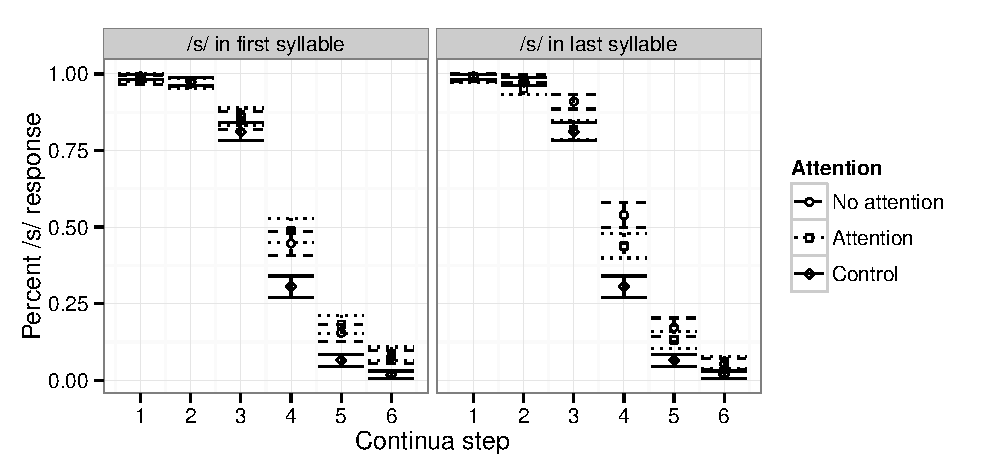
\includegraphics[width=\textwidth]{categresults}
\end{center}
\end{figure*}

One hundred and forty English words and 100 nonwords that were phonologically licit in English were used as exposure materials.  The set of words consisted of 40 critical items, 20 control items and 60 filler words.  Half the control items had an /ʃ/ in the onset of the first syllable (e.g., \emph{shoulder}) and half had an /ʃ/ in the onset of the final syllable (e.g., \emph{cushion}).  All critical tokens formed nonwords if their /s/ was replaced with /ʃ/.  Each critical item and control item contained just the one sibilant, with no /s z ʃ ʒ tʃ dʒ/.  Filler words and nonwords did not contain any sibilants. Four minimal pairs were selected as test items for categorization (\emph{sack}-\emph{shack}, \emph{sigh}-\emph{shy}, \emph{sin}-\emph{shin}, \emph{sock}-\emph{shock}).  Two of the pairs had a higher frequency in SUBTLEXus \cite{Brysbaert2009} for the /s/ word, and two had higher frequency for the /ʃ/ word.

All words and nonwords were recorded by a male who was a native speaker of the local accent. Critical words for the exposure phase were recorded in pairs, once normally and once with the sibilant swapped forming a nonword.  The speaker was instructed to produce both forms with comparable speech rate, speech style, and prosody.

For each critical item, the word and nonword versions were morphed together in an 11-step continuum (0\%-100\% of the nonword /ʃ/ recording, in steps of 10\%) using STRAIGHT \cite{Kawahara2008}.  Prior to morphing, the word and nonword versions were time-aligned based on acoustic landmarks, like stop bursts, onset of F2, nasalization or frication, etc.  All control items and filler words were processed and resynthesized by STRAIGHT to ensure consistent quality across stimulus items.  A pretest for both the exposure and categorization stimuli was performed to find the 50\% cross over point for each continuum.  For the exposure continua, the step closest to 50\% crossover was used as the exposure stimuli for that item, and for the categorization continua, three steps on either side of the cross over point were used as stimuli for categorization.

\subsection{Procedure}
Participants in the experimental conditions completed an exposure task and a categorization task.  The exposure task was lexical decision, where participants heard auditory stimuli and were instructed to respond with either ``word'' or ``nonword'', with buttons counterbalanced across participants. Trial order was pseudorandom, with no critical or control items appearing in the first six trials, and no critical or control trials in a row, following \cite{Reinisch2013}.

In the categorization task, participants heard an auditory stimulus and had to categorize it as one of two words, differing only in the onset sibilant (/s/ or /ʃ/), with buttons again counterbalanced across participants.  The six most ambiguous steps of the minimal pair continua were used with seven repetitions each, giving a total of 168 trials. Participants were instructed that there would be two tasks in the experiment, and both tasks were explained at the beginning to remove experimenter interaction between exposure and categorization, although the nature of what types of sounds were to be categorized was not revealed to participants at this time.  

Participants were assigned to one of four conditions, with two binary factors for Exposure Type (S-Initial, S-Final) and Attention (No Attention, Attention).  Participants in the S-Initial conditions were exposed to only critical items that began with /s/, and participants in the S-Final condition were exposed only to critical items that had an /s/ in the onset of the final syllable, giving a consistent 200 trials in all exposure phases with control and filler items shared across all participants.  Participants in the Attention conditions received additional instructions that the speaker's ``s'' sounds were sometimes ambiguous and to listen carefully to ensure correct responses in the lexical decision, but participants in the No Attention conditions received no such instructions.  Participants in the Control group completed the categorization task, but not the exposure task.

\section{Results}

\subsection{Exposure}

Trials with nonword stimuli and responses faster than 200 ms or slower than 2500 ms were excluded from analysis. Performance on the exposure task was high overall, with accuracy on filler trials averaging 92\%.  Word response rates for each of the four conditions did not differ significantly from each other, though S-Final/No Attention participants had a slightly higher average rate of 81\% (SD= 17\%) than the other conditions (S-Final/Attention: mean = 74\%, SD = 18\%; S-Initial/No Attention: mean = 74\%, SD = 27\%; S-Initial/Attention: mean = 76\%, SD = 23\%).  A logistic mixed effects model with accuracy as the dependent variable was fit with fixed effects for trial type (Filler, S, SH), Attention (No Attention, Attention), Exposure Type (S-Initial, S-Final) and their interactions. The random effect structure was as maximally specified as possible with random effects for Subject and Word, and by-Subject random slopes for trial type and by-Word random slopes for Attention. The only fixed effects that were significant were a main effect of trial type for /s/ trials compared to filler trials ($\beta = -1.71, SE = 0.43, z = -3.97, p < 0.01$) and a main effect of Attention ($\beta = 0.76, SE = 0.38, z = 2.02,   p = 0.04$).  Trials containing an ambiguous /s/ were less likely to be responded to as a word, and participants instructed to pay attention to /s/ were more likely to correctly respond to words in general.

\subsection{Categorization}

Responses with reaction times less than 200 ms or greater than 2500 ms were excluded from analyses. Participants were excluded if their initial estimated cross over point for the continuum lay outside of the 6 steps presented (2 participants).  A logistic mixed effects model was constructed with Subject and Continua as random effects and continua Step as random slopes, with 0 coded as a /ʃ/ response and 1 as a /s/ response.  Fixed effects for the model were Step, Exposure Type, Attention and their interactions.

There was a significant effect for the intercept ($\beta = 0.83, SE = 0.31, z = 2.6, p < 0.01$), indicating that participants categorized more of the continua as /s/ in general.  There was also a significant main effect of Step ($\beta = -2.10, SE = 0.20, z = -10.3, p < 0.01$), and a significant interaction between Exposure Type and Attention ($\beta = -0.93, SE = 0.43, z = -2.14, p = 0.03$).  There was a marginal main effect of Exposure Type ($\beta =0.58, SE = 0.30, z = 1.8, p = 0.06$).  For a similar model with Control participants, with the same random effect structure and only Step as a fixed effect, the intercept was not significant ($\beta = 0.43, SE = 0.29, z = 1.5, p = 0.13$), and Step was significant ($\beta = -2.61, SE = 0.28, z = -9.1, p < 0.01$).

These results are shown in Figure~\ref{fig:categ}.  The solid lines show the control participants' categorization function across the 6 steps of the continua.  The error bars show within-subject 95\% confidence intervals at each step.  When exposed to ambiguous /s/ tokens in the first syllables of words, participants show a general expansion of the /s/ category, but no differences in behaviour if they are warned about ambiguous /s/ productions.  However, when the exposure is to ambiguous /s/ tokens later in the words, we can see differences in behaviour beyond the general /s/ category expansion.  Participants not warned of the speaker's ambiguous tokens categorized more of the continua as /s/ than those who were warned of the speaker's ambiguous /s/ productions.

\begin{figure}[!ht]

\caption{Correlation of crossover point in categorization with the proportion of word responses to critical items containing an ambiguous /s/ token.}\label{fig:xover}
\begin{center}
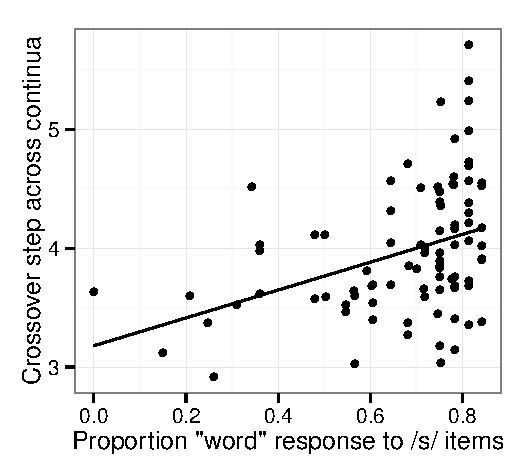
\includegraphics[width=80mm]{xoverwordresp}
\end{center}
\end{figure}

As an individual predictor of participants' performance we took the proportion critical word endorsements and compared these values to the estimated cross-over points. The crossover point was determined from the Subject random effect in the logistic mixed effects model \cite{Kleber2011}. There was a significant positive correlation between a participant's tolerance for the ambiguous exposure items and their crossover point on the continua ($r = 0.39, t (90) = 4, p < 0.01$), shown in Figure~\ref{fig:xover}.

\section{Discussion and conclusion}

Perceptual learning effects in this experiment were robust across continua and experimental conditions, indicating the general automaticity of perceptual adaptation, but the degree of adaptation differed across conditions. In the current results, differences in attention only had an effect in the S-Final conditions, which replicates earlier findings that the effect of attention increased as the position of the ambiguous sound moved toward the end of the word \cite{Pitt2012}.  The initial sound of a word is already a prominent position and listeners focus on the initial sounds to narrow the set of possible words they might be hearing. Later in a word, expectations for particular words given the preceding phonetic content would be greater, so directed attention on the phonetic detail shows a clear effect.  That attention affected perceptual learning at all suggests that the adaptation is not wholly automatic and there is some degree of listener control.

The correlation between word response rate in the exposure phase and the category boundary in categorization phase raises two possible explanations. In a causal interpretation between exposure and categorization, as each ambiguous sound is linked to a word and a phonetic category, the distribution for that category (for that particular speaker) is updated. Participants who linked more of the ambiguous sound to the /s/ category updated their perceptual category for /s/ more. This explanation fits within a larger neo-generative model of spoken language processing \cite{Pierrehumbert2002}.  A non-causal story is also plausible:  the correlation may reveal individual differences on the part of the participants, where some participants are more adaptable or tolerant of variability than others, leading to greater degrees of perceptual adaptation. The lack of learning with nonwords \cite{Norris2003} makes the latter interpretation particularly appealing. 

Perceptual learning underscores the dynamicity of the speech perception system, and these results further underscore the flexible nature of the adaptation process. Listeners adapt to varying degrees, and it is a process that is affected by context, attention, and tolerance of pronunciation variation.
 

\bibliographystyle{icphs2015}
\bibliography{icphs2015}

\end{document}
